\chapter{Transfer Integrals}

\section{Semi-empirical}

\section{Density-functional}
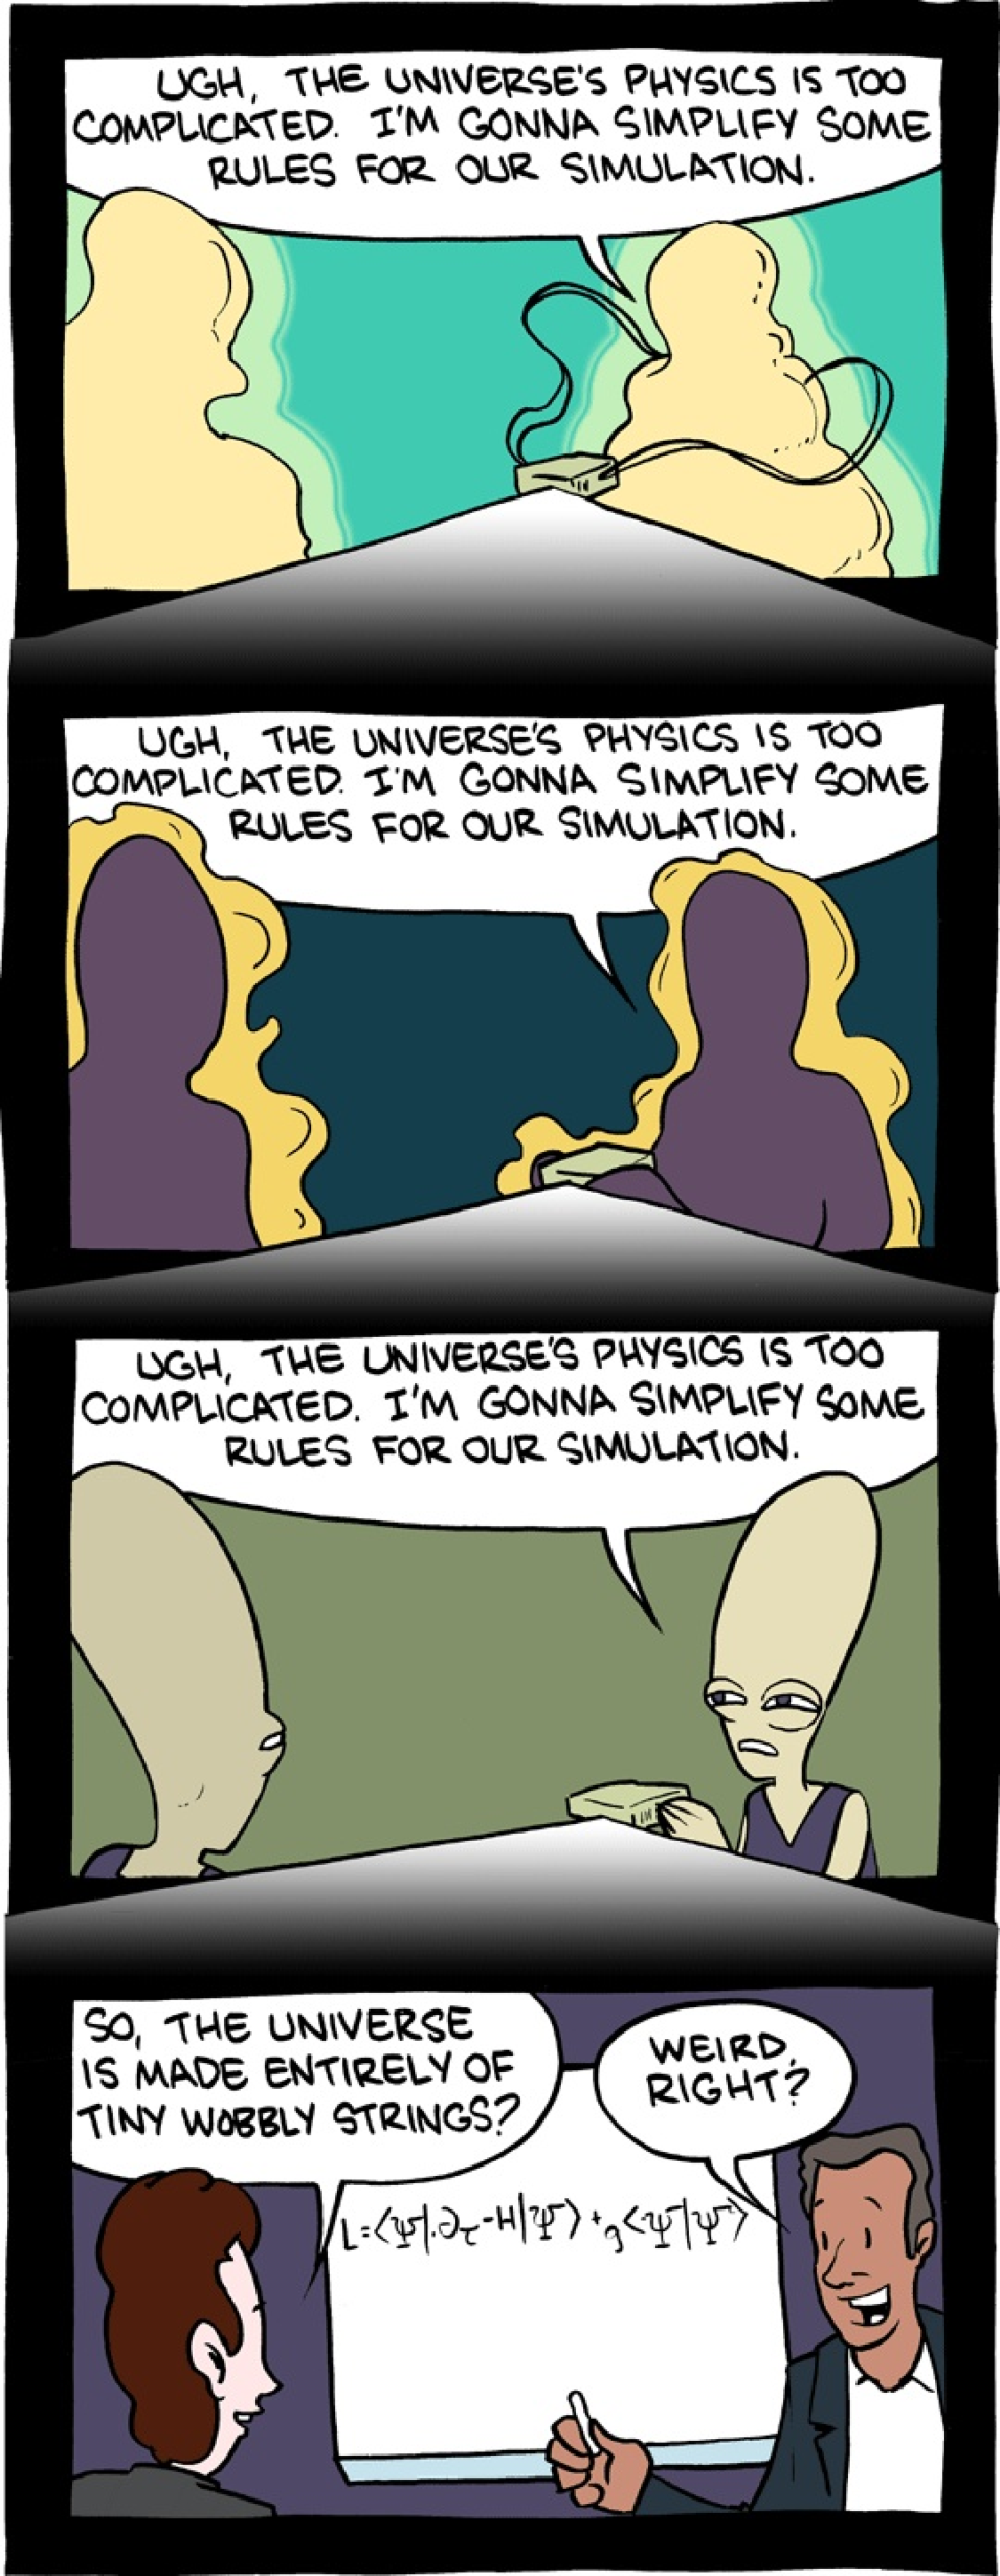
\includegraphics[width=0.4\linewidth]{fig/complicated}
\begin{itemize}
\item {\it not sure about directory structure yet, using {\tt
      \$DIRECTORY} for the time being}
\item creating file structure for frame $N$ (raw: no postpocessing,
  min: MD energy minimization) in directory {\tt OUTDIR}
\begin{verbatim}
$DIRECTORY/perpare.sh raw/min N OUTDIR
cd OUTDIR
$DIRECTORY/pairdump.sh
\end{verbatim}
\item make sure QCP environments are set!
\item running calculations for all monomers
 \begin{verbatim}
$DIRECTORY/calc_monomer QCP [METHOD]

QCP:   G for Gaussian09
       T for Turbomole

METHOD: func/basis (optional)
        overrides default functional/basisset combination
        defaults: pbepbe/6-311G** Gaussian09
                  b-p/def-TZVP    Turbomole
\end{verbatim}
\item check monomer calculations (Gaussian version to test!) 
\begin{verbatim}
$DIRECTORY/check_mols N M QCP

N:   First monomer to test
M:   Last monomer to test
QCP: G/T 
\end{verbatim}
incomplete monomers are written to file {\tt TROUBLE.mol}
\item running calculations for all dimers
 \begin{verbatim}
$DIRECTORY/calc_dimer_noSCF QCP [METHOD]

QCP:   G for Gaussian09
       T for Turbomole

METHOD: func/basis (optional)
        overrides default functional/basisset combination
        defaults: pbepbe/6-311G** Gaussian09
                  b-p/def-TZVP    Turbomole
\end{verbatim}
\item should we add {\tt trajectory\_submit.sh} that does all monomer
  and dimer calculations on the cluster (MPIP-specific)?
\end{itemize}
